% Chapter Chapter 3 For Reproducible Research in R and RStudio
% Christopher Gandrud
% Created: 16/07/2012 05:45:03 pm CEST
% Updated: 4 September 2012




\chapter{Getting Started with R, RStudio, and knitr}\label{GettingStartedRKnitr}

If you have rarely or never used R before the first two sections of this chapter give you enough information to be able to get started and understand the code I use in this book. For more detailed introductions to R please refer to the related resources I mentioned in Chapter \ref{WhatNot}. Experienced R users might want to skip the first two sections of the chapter. This chapter also gives a brief overview of RStudio. It highlights the key features of main RStudio panel (what appears when you open RStudio) and some of its key features for reproducible research. Finally, I discuss the basics of the {\emph{knitr}} package and how it is integrated into RStudio.

%%%%%%%%%%%%% Using R
\section{Using R: the basics}

As a computer language, R has FILL in

This section covers some of the very basic syntax in R to get you started. If you have little experience with R, reading this section will make it much easier for you to follow along with the examples in the book. I cover the key components of the R language including:

\begin{itemize}
    \item objects \& assignment,
    \item component selection,
    \item functions and commands,
    \item arguments,
    \item libraries.
\end{itemize}

Before discussing each of these components let's open up R and look around.\footnote{Please see Chapter \ref{Intro} for instructions on how to install R.} When you open up R you should get a window that looks something like what you see in Figure \ref{RBlankMain}.\footnote{This figure and almost all screenshots in this book are from a computer using the Mac OS 10.8 operating system.} This window is the {\bf{R console}}\index{R console}. Under the session\index{session information} information--what version of R you are using, your workspace, and so on--you should see a {\tt{\textgreater}}. This prompt is where you enter R code.\footnote{If you are using a Unix-like system such as Ubuntu or Mac OS 10, you can an application called the Terminal\index{Terminal}. If you have installed R on your computer you can type {\tt{r}} into the terminal and then the {\tt{Enter}} or {\tt{Return}} key it will begin a new R session. You know if a new R session has started if you get the same startup information is printed in the Terminal window.} To run R code that you have typed into the console type the {\tt{Enter}} or {\tt{Return}} key. Now that we have a new R session open we can get started. 

\begin{figure}[th!]
    \caption{R Startup Console}
    \label{RBlankMain}
    \begin{center}
    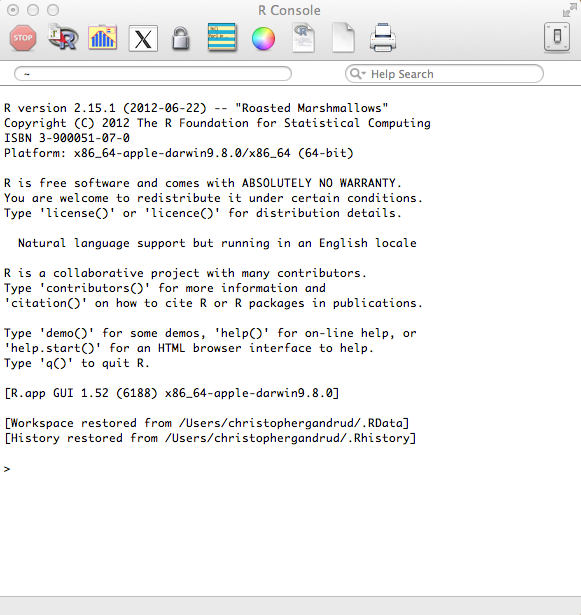
\includegraphics[scale=0.4]{/git_repositories/Rep-Res-Book/Source/Children/Chapter3/images3/BlankRConsole.png}
    \end{center}
\end{figure}

\subsection{Objects}\label{Objects}

You will probably have read that `R is an object-oriented\index{object-oriented} language'.  What are objects? Objects are like the R language's nouns. They are things, such as a list of numbers, a data set, a word, a table of results from some analysis, and so on. Saying that R is `object-oriented' just means that R is focused on doing actions to objects. We will talk about the actions--commands and functions--later in this section. For now let's create a few objects.

\paragraph{Numeric \& string objects}

Different types of objects have different data types or modes\index{mode}. Let's make two basic objects of the numeric and character mode. We can choose almost any name we want for our objects.\footnote{Objects must begin with an alphabetic character and cannot have spaces.} Let's call our numeric object {\emph{Number}}. To put something into the object we use the {\bf{assignment operator}}: {\tt{\textless -}}. Let's assign the number 10 to our Number object.

\begin{knitrout}
\definecolor{shadecolor}{rgb}{0.969, 0.969, 0.969}\color{fgcolor}\begin{kframe}
\begin{alltt}
Number <- 10
\end{alltt}
\end{kframe}
\end{knitrout}


\noindent To see the contents of our object, just type its name.

\begin{knitrout}
\definecolor{shadecolor}{rgb}{0.969, 0.969, 0.969}\color{fgcolor}\begin{kframe}
\begin{alltt}
Number
\end{alltt}
\begin{verbatim}
## [1] 10
\end{verbatim}
\end{kframe}
\end{knitrout}


\noindent Lets's briefly breakdown this output. \texttt{10} is clearly the contents of {\emph{Number}}. The double hash (\texttt{\#\#}) is included in the output by {\emph{knitr}} to tell you that this is output rather than R code.\footnote{This makes it easier to copy and past code included in a presentation document by {\emph{knitr}}.} Finally, \texttt{[1]} is the row number of the object that 10 is on. Clearly our object only has one row.   

Creating a character object is very similar. The only difference is that we enclose the character string (letters in a word for example) inside of quotation marks ({\tt{""}}). To create an object called {\emph{Words}} that contains a character string ``Hello World".\label{StringObject}

\begin{knitrout}
\definecolor{shadecolor}{rgb}{0.969, 0.969, 0.969}\color{fgcolor}\begin{kframe}
\begin{alltt}
Words <- \hlstring{"Hello World"}
\end{alltt}
\end{kframe}
\end{knitrout}



An object's class is important to keep in mind as it determines what things we can do to it. For example you cannot take the mean of a character mode object like the {\emph{Words}} object we created earlier:

\begin{knitrout}
\definecolor{shadecolor}{rgb}{0.969, 0.969, 0.969}\color{fgcolor}\begin{kframe}
\begin{alltt}
\hlfunctioncall{mean}(Words)
\end{alltt}


{\ttfamily\noindent\textcolor{warningcolor}{\#\# Warning: argument is not numeric or logical: returning NA}}\begin{verbatim}
## [1] NA
\end{verbatim}
\end{kframe}
\end{knitrout}


\noindent Trying to find the mean of our {\emph{Words}} object gave us a warning message and returned the value {\tt{NA}}\index{NA}: not applicable. You can also think of {\tt{NA}} to mean missing. To find out what class an object has use the {\tt{class}} command. For example:

\begin{knitrout}
\definecolor{shadecolor}{rgb}{0.969, 0.969, 0.969}\color{fgcolor}\begin{kframe}
\begin{alltt}
\hlfunctioncall{class}(Words)
\end{alltt}
\begin{verbatim}
## [1] "character"
\end{verbatim}
\end{kframe}
\end{knitrout}


\paragraph{Vector \& data frame objects}

Sp far we have only looked at objects with a single number or string.\footnote{These might be called scalar objects, though in R scalars are just vectors with a length of 1.} Clearly we want to be using objects--data sets--that have many strings and numbers. In R these are usually {\bf{data frame}}\index{data frame} type objects and are roughly equivalent to the type of data structure you would be familiar with from using a program such as Microsoft Excel. We will be using data frames extensively throughout the book. It is also useful to cover other, simpler types of objects, primarily vectors. Vectors are R's ``workhorse".\cite{Matloff2011} Knowing how to use vectors\index{vector} will be especially helpful when we clean up raw data in Chapter \ref{DataClean} and make tables in Chapter \ref{TablesChapter}.\footnote{If you want information about other types of R objects such as lists\index{list} and matrices\index{matrix}, Chapter 1 of Norman Matloff's book\cite{Matlof2011} is a really good place to look.} \\[0.25cm]

\noindent {\bf{Vectors}}: \\[0.25cm] Vectors are the ``fundamental data type"\cite{Matloff2011} in R. They are simply an ordered group of numbers, character strings, and so on.\footnote{In a vector every member of the group must be of the same type. Lists are similar to vectors, but allow you to have different types.} It may be useful to think of basically all other data types as complicated forms of vectors. For example, data frames are basically multiple vectors of the same length--i.e. they have the same number of rows--and possibly of different types attached together. 

Let's create a very simple numeric vector containing the numbers 2.8, 2, and 14.8. To do this we will use the \texttt{c} (concatenate)\index{concatenate} function:

\begin{knitrout}
\definecolor{shadecolor}{rgb}{0.969, 0.969, 0.969}\color{fgcolor}\begin{kframe}
\begin{alltt}
NumericVect <- \hlfunctioncall{c}(2.8, 2, 14.8)

\hlcomment{# Show NumericVect's contents}
NumericVect
\end{alltt}
\begin{verbatim}
## [1]  2.8  2.0 14.8
\end{verbatim}
\end{kframe}
\end{knitrout}


Vectors of character strings are created in a similar way. The only major difference is that each character string is enclosed in quotation marks like this:

\begin{knitrout}
\definecolor{shadecolor}{rgb}{0.969, 0.969, 0.969}\color{fgcolor}\begin{kframe}
\begin{alltt}
CharacterVect <- \hlfunctioncall{c}(\hlstring{"Albania"}, \hlstring{"Botswana"}, \hlstring{"Cambodia"})

\hlcomment{# Show CharacterVect's contents}
CharacterVect
\end{alltt}
\begin{verbatim}
## [1] "Albania"  "Botswana" "Cambodia"
\end{verbatim}
\end{kframe}
\end{knitrout}


To give you a preview of what we are going to do when we start working with real data sets, lets combine the two vectors {\emph{NumericVect}} and {\emph{CharacterVect}} into a new object with the \texttt{cbind}\index{cbind} function. This function binds the two vectors together as if they were different columns.\footnote{If you want to combine objects as if they were rows of the same column(s) use the \texttt{rbind} function.}

\begin{knitrout}
\definecolor{shadecolor}{rgb}{0.969, 0.969, 0.969}\color{fgcolor}\begin{kframe}
\begin{alltt}
StringNumObject <- \hlfunctioncall{cbind}(CharacterVect, NumericVect)

\hlcomment{# Show StringNumObject's contents}
StringNumObject
\end{alltt}
\begin{verbatim}
##      CharacterVect NumericVect
## [1,] "Albania"     "2.8"      
## [2,] "Botswana"    "2"        
## [3,] "Cambodia"    "14.8"
\end{verbatim}
\end{kframe}
\end{knitrout}


\noindent By binding these two objects together we've created a new matrix\index{matrix} object.\footnote{Matrices are vectors with columns as well as rows.} You can see that the numbers in the {\emph{NumericVect}} column are between quotation marks. Matrices, like vectors can only have one data type or mode. 

\noindent {\bf{Data frames}}: If we want to have an object with rows and columns and allow the columns to contain data with different modes, we need to use data frames\index{data frame}. Let's use the \texttt{data.frame} command to combine the {\emph{NumericVect}} and {\emph{CharacterVect}} objects.

\begin{knitrout}
\definecolor{shadecolor}{rgb}{0.969, 0.969, 0.969}\color{fgcolor}\begin{kframe}
\begin{alltt}
StringNumObject <- \hlfunctioncall{data.frame}(CharacterVect, NumericVect)

\hlcomment{# Display contents of StringNumObject data frame}
StringNumObject
\end{alltt}
\begin{verbatim}
##   CharacterVect NumericVect
## 1       Albania         2.8
## 2      Botswana         2.0
## 3      Cambodia        14.8
\end{verbatim}
\end{kframe}
\end{knitrout}


\noindent There are two important things to notice. The first is that because we used the same name for the data frame object as the previous matrix object, R deleted the matrix object and completely replaced it with the data frame. This is something to keep in mind when you are creating new objects. You will also notice that the strings in the {\emph{CharacterVect}} object no longer are in quotation marks. This does not mean, however that they are no longer character string type data. To prove this try taking the mean of {\emph{CharacterVect}} like this:

\begin{knitrout}
\definecolor{shadecolor}{rgb}{0.969, 0.969, 0.969}\color{fgcolor}\begin{kframe}
\begin{alltt}
\hlfunctioncall{mean}(StringNumObject$ChacterVect)
\end{alltt}


{\ttfamily\noindent\textcolor{warningcolor}{\#\# Warning: argument is not numeric or logical: returning NA}}\begin{verbatim}
## [1] NA
\end{verbatim}
\end{kframe}
\end{knitrout}


\subsection{Component Selection}

The last bit of code will probably be confusing. Why do we have a dollar sign (\texttt{\$}) inbetween the name of our data frame object and the character column? The dollar sign is called the component selector\index{component selection}. It basically extracts a part of an object. In the previous example it extracts the {\emph{
CharacterVect}} column from the {\emph{StringNumObject}} and feeds this to the \texttt{mean} command, which tries (in this case unsuccessfully) to find its mean.

We can of course use the component selector to create new objects with parts of other objects. Imagine that we only have the {\emph{StringNumObject}}, but want an object with only the information in the numbers column. Let's the following code:

\begin{knitrout}
\definecolor{shadecolor}{rgb}{0.969, 0.969, 0.969}\color{fgcolor}\begin{kframe}
\begin{alltt}
NewNumeric <- StringNumObject$NumericVect

\hlcomment{# Display contents of NewNumeric}
NewNumeric
\end{alltt}
\begin{verbatim}
## [1]  2.8  2.0 14.8
\end{verbatim}
\end{kframe}
\end{knitrout}


\noindent Knowing how to use the component selector will be especially useful when we discuss making tables for presentation documents in Chapter \ref{TablesChapter}.

\subsection{Subscripts}

Another way to select parts of an object is to use subscripts\index{subscripts}. These are denoted with square braces (\texttt{[]}). We can use them to select not only columns from data frames but also rows and individual cells. As we began to see in some of the previous output, each part of a data frame as an address captured by its row and column number. We can tell R to find a part of an object by putting the row number, column number/name, or both in square braces. The first part denotes the rows and separated by a comma (\texttt{,}) are the columns. 

To give you an idea of how this works lets use the {\emph{cars}} data set that comes with R. Use the \texttt{head} command to get a sense of what this data set looks like.

\begin{knitrout}
\definecolor{shadecolor}{rgb}{0.969, 0.969, 0.969}\color{fgcolor}\begin{kframe}
\begin{alltt}
\hlfunctioncall{head}(cars)
\end{alltt}
\begin{verbatim}
##   speed dist
## 1     4    2
## 2     4   10
## 3     7    4
## 4     7   22
## 5     8   16
## 6     9   10
\end{verbatim}
\end{kframe}
\end{knitrout}


\noindent Here we can see a data frame with information on various cars speed ({\emph{speed}}) and distance ({\emph{dist}}). If we want to select only the third through seventh rows we can use the following subscript commands:

\begin{knitrout}
\definecolor{shadecolor}{rgb}{0.969, 0.969, 0.969}\color{fgcolor}\begin{kframe}
\begin{alltt}
cars[3:7, ]
\end{alltt}
\begin{verbatim}
##   speed dist
## 3     7    4
## 4     7   22
## 5     8   16
## 6     9   10
## 7    10   18
\end{verbatim}
\end{kframe}
\end{knitrout}


\noindent To select the fourth row of the {\emph{dist}} column we can type:

\begin{knitrout}
\definecolor{shadecolor}{rgb}{0.969, 0.969, 0.969}\color{fgcolor}\begin{kframe}
\begin{alltt}
cars[4, 2]
\end{alltt}
\begin{verbatim}
## [1] 22
\end{verbatim}
\end{kframe}
\end{knitrout}


\noindent An equivalent way to do this is:

\begin{knitrout}
\definecolor{shadecolor}{rgb}{0.969, 0.969, 0.969}\color{fgcolor}\begin{kframe}
\begin{alltt}
cars[4, \hlstring{"dist"}]
\end{alltt}
\begin{verbatim}
## [1] 22
\end{verbatim}
\end{kframe}
\end{knitrout}


\subsection{Functions and commands}

If objects are the nouns of the R language functions and commands\footnote{For the purposes of this book I treat the two as the same.} are the verbs. They do things to objects. Let's use the \texttt{mean} command as an example. This command takes the mean of a numeric vector object. Remember our {\emph{NumericVect}} object from before:

\begin{knitrout}
\definecolor{shadecolor}{rgb}{0.969, 0.969, 0.969}\color{fgcolor}\begin{kframe}
\begin{alltt}
\hlcomment{# Show contents of NumericVect}
NumericVect
\end{alltt}
\begin{verbatim}
## [1]  2.8  2.0 14.8
\end{verbatim}
\end{kframe}
\end{knitrout}


\noindent To find the mean of this object simply type:

\begin{knitrout}
\definecolor{shadecolor}{rgb}{0.969, 0.969, 0.969}\color{fgcolor}\begin{kframe}
\begin{alltt}
\hlfunctioncall{mean}(x = NumericVect)
\end{alltt}
\begin{verbatim}
## [1] 6.533
\end{verbatim}
\end{kframe}
\end{knitrout}


\noindent We use the assignment operator to place a command's output into an object. For example,

\begin{knitrout}
\definecolor{shadecolor}{rgb}{0.969, 0.969, 0.969}\color{fgcolor}\begin{kframe}
\begin{alltt}
MeanNumericVect <- \hlfunctioncall{mean}(x = NumericVect)
\end{alltt}
\end{kframe}
\end{knitrout}


\noindent Notice that we typed the command's name then enclosed the object name in parentheses immediately afterwards. This is the basic sytax that all commands take: \texttt{COMMAND(ARGUMENTS)}. 

\subsection{Arguments}

Arguments modify what commands do. In this example we have given the \texttt{mean} command one argument (\texttt{x = NumericVect}) telling it that we want to find the mean of NumericVect. Arguments use the \texttt{ARGUMENT LABEL = VALUE} syntax.\footnote{Note: you do not have to put spaces between the argument label and the equals sign or the equals sign and the value. However, having spaces can make your code easier for other people to read.} To find all of the arguments that an argument can accept look at the {\emph{Arguments}} section of the commands help file\index{help file}. To access the help file type: \texttt{?COMMAND}. For example,

\begin{knitrout}
\definecolor{shadecolor}{rgb}{0.969, 0.969, 0.969}\color{fgcolor}\begin{kframe}
\begin{alltt}
?mean
\end{alltt}
\end{kframe}
\end{knitrout}


\noindent The help file will also tell you the default values that the arguments are set at. Clearly, you do not need to explicitly set an argument if you want it's default value.

Let's see how to use multiple arguments for one command with the \texttt{round} command. It rounds a vector of numbers. We can use the \texttt{digits} option to specify how many decimal places we want the numbers rounded to. For example, to round the object {\emph{MeanNumericVect} to one decimal place type:

\begin{knitrout}
\definecolor{shadecolor}{rgb}{0.969, 0.969, 0.969}\color{fgcolor}\begin{kframe}
\begin{alltt}
\hlfunctioncall{round}(x = MeanNumericVect, digits = 1)
\end{alltt}
\begin{verbatim}
## [1] 6.5
\end{verbatim}
\end{kframe}
\end{knitrout}


\noindent You can see that arguments are separated by commas. 

Arguments for logical arguments must written as \texttt{TRUE} or \texttt{FALSE}.\footnote{They can be abbreviated \texttt{T} and \texttt{F}.} Arguments that are character strings should be in quotation marks.

Some arguments do not need to be explicitly labelled. For example we could have written:

\begin{knitrout}
\definecolor{shadecolor}{rgb}{0.969, 0.969, 0.969}\color{fgcolor}\begin{kframe}
\begin{alltt}
\hlcomment{# Find mean of NumericVect}
\hlfunctioncall{mean}(NumericVect)
\end{alltt}
\begin{verbatim}
## [1] 6.533
\end{verbatim}
\end{kframe}
\end{knitrout}


\noindent R will do its best to figure out what you want and will only give up when it can't--producing an error message. However, to avoid any misunderstandings between yourself and R it can be good practice to label all of your arguments. This will also make your code easier for other people to read, i.e. it will be more reproducible.

Finally, you can stack arguments inside of other arguments. To have R find the mean of NumericVect and round it to one decimal place use:

\begin{knitrout}
\definecolor{shadecolor}{rgb}{0.969, 0.969, 0.969}\color{fgcolor}\begin{kframe}
\begin{alltt}
\hlfunctioncall{round}(\hlfunctioncall{mean}(NumericVect), digits = 1)
\end{alltt}
\begin{verbatim}
## [1] 6.5
\end{verbatim}
\end{kframe}
\end{knitrout}


\subsection{Installing new libraries and loading commands}

You can install new add-on packages\index{packages}\label{Packages} using the {\tt{install.packages}}\index{install.packages} command. By default this command downloads and installs the packages from the Comprehensive R Archive Network (CRAN)\index{CRAN}. For the code you will need to install all of the package libraries used in this book see \ref{ReqPackages}.

Commands are stored in R libraries\index{R libraries}. R automatically loads a number of basic libraries by default. One of the great things about R is the many user-created libraries\footnote{For the latest list see: \url{http://cran.r-project.org/web/packages/available_packages_by_name.html}} that greatly expand the number of commands we can use. To load a library so that you can use its functions use the \texttt{library} command. Use the following code to load the {\emph{ggplot2}} library that we use in Chapter \ref{FiguresChapter} to create figures.

\begin{knitrout}
\definecolor{shadecolor}{rgb}{0.969, 0.969, 0.969}\color{fgcolor}\begin{kframe}
\begin{alltt}
\hlfunctioncall{library}(ggplot2)
\end{alltt}
\end{kframe}
\end{knitrout}


\noindent Please note that I only specify the library a command is in if the library is not loaded by default when you start an R session. 

%%%%%%%%%%%%%%% Using RStudio
\section{Using RStudio}

As I mentioned in Chapter \ref{Intro}, RStudio is an integrated development environment. It provides a centralized and well organized place to do almost anything you want to do with R. As we will see later in this chapter it is especially well integrated with literate programming tools for reproducible research. Right now let's just take a quick tour of the basic RStudio window.

\paragraph{The default window}

When you first open RStudio\index{RStudio} you should get a default window that looks like Figure \ref{BlankMain}. In this figure you see three window panes\index{RStudio pane}. The large one on the left is the {\emph{Console}}. This pane functions exactly the same as the console in regular R. Other panes include the {\emph{Workspace/History}} panes, usually in the upper right-hand corner. The Workspace pane keeps a record of all of the objects in your current workspace. You can click on an object in this pane to see its contents. This is especially useful for quickly looking at a data set in much the same way that you can scan a Microsoft Excel spreadsheet. The History pane records all of the commands you have run. It allows you to rerun code and insert it into a source code file.

\begin{figure}[ht]

    \caption{RStudio Startup Panel}
    \label{BlankMain}
    \begin{center}
    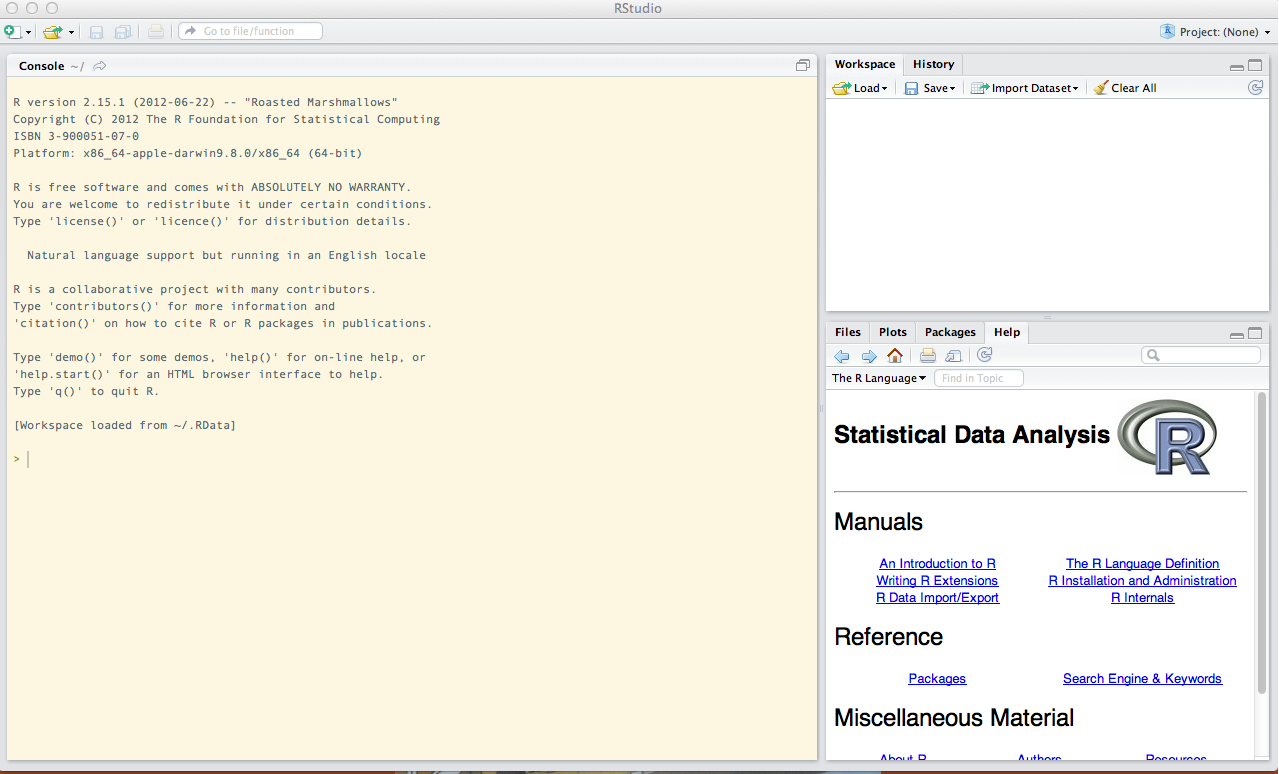
\includegraphics[width = \textwidth]{/git_repositories/Rep-Res-Book/Source/Children/Chapter3/images3/BlankMainPanel.png}
    \end{center}
\end{figure}

In the lower right-hand corner you will see the {\emph{Files/Plots/Packages/Help}} pane. We will discuss the Files pane in more detail in Chapter \ref{DirectoriesChapter}. Basically, it allows you to see and organize your files. The Plots pane is where figures you create in R will appear. This pane allows you to see all of the figures you have created in a session using the right and left arrow icons. It also lets you save the figures in a variety of formats. The Packages pane shows the packages you have installed, allows you to load individual packages by clicking on the dialog box next to them, access their manual files (click on the package name), update the packages, and even install new packages. Finally, the Help pane shows you help files. You can search for help files and search within help files using this pane.  

\paragraph{The source pane}

There is an important pane that does not show up when you open RStudio for the first time. This is the Source pane. The Source pane is where you create, edit, and run your source code files. It also functions as an editor for your markup files. It is the center of reproducible research in RStudio. Let's first look at how to use the Source pane with regular R files. These have the file extension \texttt{.R}.

You can create a new source code document, which will open a new Source pane, by going to \texttt{File} \textrightarrow \: \texttt{New}. In this drop down menu you have the option to create a variety of different source code documents. Select the \texttt{R Source} option. You should now see a new pane with a bar across the top like the first image in Figure \ref{SourcePanes}. To run the R code you have in your source code file simply highlight it\footnote{If you are only running one line of code you don't need to highlight the code, you can simply put your cursor on that line.} and click the \texttt{Run} icon on the top bar. This sends the code to the console where it is executed. The icon next to the right of \texttt{Run} simply runs the code above where you have highlighted. The \texttt{Source} icon next to this runs all of the code in file using R's \texttt{source} command\index{source command}. The icon next to \texttt{Source} is for compiling RStudio notebooks. We will look at creating notebooks later in this chapter.

We will cover how to use the Source pane with literate programming file formats--e.g. R Markdown and R LaTeX--in more detail after first discussing the {\emph{knitr}} basics. 

\begin{figure}[ht]
    \caption{RStudio Source Code Pane Top Bars}
    \label{SourcePanes}
    \begin{center}
    
        \begin{subfigure}
            \caption{R Source Code}
            
\includegraphics[width = \textwidth]{/git_repositories/Rep-Res-Book/Source/Children/Chapter3/images3/RSourceBar.png}
        \end{subfigure}\\[0.5cm]
        
        \begin{subfigure}
            \caption{R Markdown Files}
            
\includegraphics[width = \textwidth]{/git_repositories/Rep-Res-Book/Source/Children/Chapter3/images3/MarkdownSourceBar.png}
        \end{subfigure}\\[0.5cm]
        
        \begin{subfigure}
            \caption{LaTeX Markdown Files}
            
\includegraphics[width = \textwidth]{/git_repositories/Rep-Res-Book/Source/Children/Chapter3/images3/LaTeXSourceBar.png}
        \end{subfigure}
        
    \end{center}
\end{figure}



%%%%%%%%%%%%% Using knitr
\section{Using knitr: the basics}

To get started with {\emph{knitr}}\index{knitr} in R or RStudio we need to learn some of the basic concepts and syntax. The concepts are the same regardless of the markup language that we are using, but much of the syntax varies.

\subsection{File extensions}

When you save a knitable file use a file extension that indicates (a) that it is knitable and (b) what markup language it is using. You can use a number of file extensions for R Markdown files including: \texttt{.Rmd} and \texttt{.Rmarkdown}. LaTeX documents that include {\emph{knitr}} code chunks are generally called R Sweave\index{R Sweave} files and have the file extension {\tt{.Rnw}}. This terminology is a little confusing. It is a holdover from {\emph{knitr}}'s main literate programming predecessor {\emph{Sweave}}.\cite{Leisch2002} You can also use the file extension \texttt{.Rtex}, which is less confusing file extension. However, the code chunk syntax for \texttt{.Rtex} files is different from that use in \texttt{.Rnw} files. We'll look at this in more detail below.

\subsection{Code Chunks}

When we want to include R code into our presentation documents we place them in a code chunk\index{code chunk}. Code chunk syntax differs depending on the markup language we are using to write our documents. Let's see the syntax for R Markdown and R LaTeX files.

\paragraph{R Markdown}

In R Markdown files we begin a code chunk by writing: \texttt{\`\`\`\\ \{r\} }. A code chunk is closed--ended--simply with: \`\`\`\ . For example:

\begin{knitrout}
\definecolor{shadecolor}{rgb}{0.969, 0.969, 0.969}\color{fgcolor}\begin{kframe}
\begin{alltt}
```\{r\}
\hlcomment{# Example of a R Markdown code chunk}
StringNumObject <- \hlfunctioncall{cbind}(CharacterVect, NumericVect)
```
\end{alltt}
\end{kframe}
\end{knitrout}


\paragraph{R LaTeX}

There are two different ways to delimite code chunks in R LaTeX documents. One way largely emulates the established {\emph{Sweave}} syntax.\footnote{The syntax originates in a literate programming tool called noweb \cite[]{Leisch2002,RamseyNoweb}.} {\emph{Knitr}} now also supports files with the {\tt{.Rtex}} extension, though the code chunk syntax is different. I will cover both types of syntax for code chunks in LaTeX documents, though in throughout the book I use the older and more established {\emph{Sweave}} style syntax. \\[0.25cm]

\noindent {\bf{Sweave-style}} \\[0.25cm]

Traditional Sweave-style code chunks begin with the following code: \texttt{\textless\textless \textgreater\textgreater=}. The code chunk is closed with an at sign (@). \\[0.25cm]

\noindent {\bf{Rtex-style}} \\[0.25cm]

Sweave-style code chunks may seem fairly baroque. Another option for LaTeX files is the Rtex-style syntax. To begin a code chunk simply type \texttt{\%\% begin.rcode}. To close the chunk you use double percent signs: \texttt{\%\%}. Each line in the code chunk needs to begin with a single percent sign. For example:

\begin{knitrout}
\definecolor{shadecolor}{rgb}{0.969, 0.969, 0.969}\color{fgcolor}\begin{kframe}
\begin{alltt}
%% begin.rcode
% \hlcomment{# Example of a Rtex-style code chunk}
% StringNumObject <- \hlfunctioncall{cbind}(CharacterVect, NumericVect)
%%
\end{alltt}
\end{kframe}
\end{knitrout}


\paragraph{Code chunk labels}

Each chunk has a label. When a code chunk creates a plot or is cached\index{cache} (see below for more details) {\emph{knitr}} uses the chunk label for the resulting file's name. If you do not explicitly give the chunk a label it will be assigned one like: \texttt{unnamed-chunk-i}. \texttt{i} is the chunk's number.

To explicitly assign chunk labels in R Markdown documents place the label name inside of the braces after the \texttt{r}. If we wanted to use the label \texttt{ChunkLabel} we would simply type this at the beginning:

\begin{knitrout}
\definecolor{shadecolor}{rgb}{0.969, 0.969, 0.969}\color{fgcolor}\begin{kframe}
\begin{alltt}
```\{r ChunkLabel\}
\hlcomment{# Example chunk label}
```
\end{alltt}
\end{kframe}
\end{knitrout}


\noindent The same general format applies to the two types of LaTeX chunks. In Sweave-style chunks we would type: \texttt{\textless\textless ChunkLabel\textgreater\textgreater=}. In Rtex-style we simply use: \texttt{\%\% begin.rcode ChunkLabel}.

Try not to use spaces or periods in your label names. And all chunk labels {\emph{must}} be unique.

\paragraph{Code chunk options}

There are many times when we want to change how our code chunks are knitted and presented. Maybe we only want to show the code and not the results or perhaps we don't want to show the code at all but just a figure that it produces. Chunk options can also be used to format the size and placement of this figure. To make these changes, and many others we can specify code chunk options\index{code chunk options}.

Like chunk labels, you specify options in the chunk head. Place them after the chunk label, separated by a comma. Chunk options are written following the same rules as arguments to regular R commands. They have the same \texttt{option=value} structure as arguments. The option values must be written in the same way that argument values are. Character strings need to be inside of quotation marks. The logical \texttt{TRUE} and \texttt{FALSE} operators cannot be written ``true" and ``false". For example, imagine we have a Markdown code chunk called \texttt{ChunkLabel}. If we only want to have {\emph{knitr}} include the code in our document, but not actually run it we use the option \texttt{eval=FALSE}. This option tells {\emph{knitr}} not to evaluate (run) the code chunk.

\begin{knitrout}
\definecolor{shadecolor}{rgb}{0.969, 0.969, 0.969}\color{fgcolor}\begin{kframe}
\begin{alltt}
```\{r ChunkLabel, eval=FALSE\}
\hlcomment{# Example of a non-evaluated code chunk}
StringNumObject <- \hlfunctioncall{cbind}(CharacterVect, NumericVect)
```
\end{alltt}
\end{kframe}
\end{knitrout}


\noindent Note that all labels and code chunk options must be on the same line. Options are separated by commas. The syntax for {\emph{knitr}} options is the same regardless of the markup language. Here is the same chunk option in Rtex-style syntax:

\begin{knitrout}
\definecolor{shadecolor}{rgb}{0.969, 0.969, 0.969}\color{fgcolor}\begin{kframe}
\begin{alltt}
%% begin.rcode ChunkLabel, eval=FALSE
% \hlcomment{# Example of a non-evaluated code chunk}
% StringNumObject <- \hlfunctioncall{cbind}(CharacterVect, NumericVect)
%%
\end{alltt}
\end{kframe}
\end{knitrout}

Throughout this book we will look at a number of different code chunk options. For the full list of {\emph{knitr}} options see the {\emph{knitr}} chunk options page maintained by {\emph{knitr}}'s creator Yihui Xie: \url{http://yihui.name/knitr/options#package_options}.

\subsection{Global Options}

So far we have only looked at how to set local options\index{local chunk options} in {\emph{knitr}} code chunks. If we want an option to apply to all of the chunks in our document we can set {\bf{global chunk options}}\index{global chunk options}. They options are `global' in the sense that they apply to the entire document. Setting global chunk options helps us create documents that are formatted consistently without having to repetitively specify the same option every time we create a new code chunk. For example, in this book I center almost all of the the figures. Instead of using the {\tt{fig.align='center'}} option in each code chunk that creates a figure I set the option globally.

To set a global option first create a new code chunk at the beginning of your document\footnote{In Markdown, you can put global chunk options at the very top of the document. In LaTeX they should be after the \texttt{\textbackslash{}begin\{document\}} command (see Chapter \ref{LatexChapter} for more information on how LaTeX documents are structured).} You will probably want to set the option {\tt{echo=FALSE}} so that {\emph{knitr}} doesn't echo the code. Inside the code chunk use {\tt{opts\_chunk\$set}}. You can set any chunk option as an argument to {\tt{opts\_chunk\$set}}. The option will be applied across your document, unless you set a different local option. 

Here is an example of how we could have all of the figures in a Markdown document created by {\emph{knitr}} code chunks center aligned. We place the following code at the beginning of the document:

\begin{knitrout}
\definecolor{shadecolor}{rgb}{0.969, 0.969, 0.969}\color{fgcolor}\begin{kframe}
\begin{alltt}
```\{r GlobalFigOpts, echo=FALSE\}
\hlcomment{# Center align all knitr figures}
opts_chunk$\hlfunctioncall{set}(fig.align=\hlstring{'center'})
```
\end{alltt}
\end{kframe}
\end{knitrout}


\subsection{knitr package options}

Chunk options determine how we want to treat code chunks. We can also set package options\index{package options} that affect how the {\emph{knitr}} package itself runs. For example, the {\tt{progress}} option can be set as either {\tt{TRUE}} or {\tt{FALSE}}\footnote{It's set as {\tt{TRUE}} by default.} depending on whether or not we want a progress bar\index{progress bar} to be displayed when we knit a code chunk.\footnote{The {\emph{knitr}} progress bar looks like this {\tt{|>>>>>>| 100\%}} and indicates how much of a code chunk has been run.} You can use {\tt{base.dir}} to set the directory where you want all of your figures to be saved to (see Chapter \ref{DirectoriesChapter}) or the {\tt{child.path}} option to specify where child documents are located (see Chapter \ref{LargeDocs}).

We set package options in a similar way to global chunk options with {\tt{opts\_knit\$set}}. For example, to turn off the progress bar when knitting Markdown documents include this code at the beginning of the document:

\begin{knitrout}
\definecolor{shadecolor}{rgb}{0.969, 0.969, 0.969}\color{fgcolor}\begin{kframe}
\begin{alltt}
```\{r GlobalFigOpts, echo=FALSE\}
\hlcomment{# Turn off knitr progress bar}
opts_knit$\hlfunctioncall{set}(progress=FALSE)
```
\end{alltt}
\end{kframe}
\end{knitrout}


%%%%%%%%%% Knitr & RStudio
\subsection{knitr \& RStudio}

RStudio is highly integrated with {\emph{knitr}} and the markup languages knitr works with. Because of this integration it is easier to create and compile {\emph{knitr}} documents than doing so in plain R. Most of the RStudio/{\emph{knitr} features are accessed in the Source pane\index{Source pane}. The Source pane's appearance and capabilities changes depending on the type of file you have open in it. RStudio uses the file extension\index{file extension} to automatically determine what type of file you have open.\footnote{You can manually set how you want the Source pane to act by selecting the file type using the drop down menu in the lower right-hand corner of the Source pane.} We have already seen some of the features the Source pane has for R source code files. Let's now look at how to use {\emph{knitr}} with R source code files as well as the markup formates we cover in this book: R Markdown\index{R Markdown}, and R LaTeX\index{R LaTeX}. \\[0.25cm]

\paragraph{Compiling R source code notebooks}

If you want a quick well formatted--i.e not a copy and pasted version of what is in the console--account of the code that you ran and the results that you got you can use RStudio's ``Compile Notebook"\index{notebook} capabilities. RStudio uses {\emph{knitr}} to create a standalone HTML file that includes all code from an R source file as well as the output. This can be useful for recording the steps you took to do an analysis. You can see an example RStudio notebook in Figure \ref{NotebookExample}. 

If you want to create a notebook from an open R source code file simply click click the \texttt{Compile Notebook} icon in the Source pane's top bar (see Figure \ref{SourcePanes}.\footnote{Alternatively, \texttt{File} \textrightarrow \; \texttt{Compile Notebook\ldots}} Then click the \texttt{Compile} button in the window that pops up. In Figure \ref{NotebookExample} you can see near the top center right a small globe icon next to the word ``Publish". Clicking this allows you to publish your notebook to RPubs (\url{http://www.rpubs.com/}). RPubs allows you to share your notebooks over the internet. You can publish not only notebooks, but also any {\emph{knitr}} Markdown document you compile in RStudio.

\begin{figure}
    \caption{RStudio Notebook Example}
    \label{NotebookExample}
    \begin{center}
    
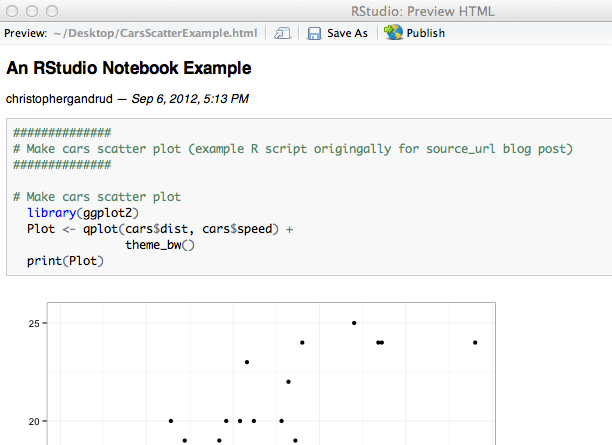
\includegraphics[scale=0.4]{/git_repositories/Rep-Res-Book/Source/Children/Chapter3/images3/NotebookExample.png}
    \end{center}
\end{figure}

\paragraph{R Markdown} The second image in figure \ref{SourcePanes} is what the Source pane's top bar looks like when you have an R Markdown file open. You'll notice the familiar \texttt{Run} button for running R code. At the far right you can see a new \texttt{Chunks} drop down menu. In this menu you can select \texttt{Insert Chunk} to insert the basic syntax required for a code chunk. There is also an option to \texttt{Run Current Chunk}--i.e. the chunk where your cursor is located--\texttt{Run Next Chunk}, and \texttt{Run All} chunks. You can navigate to a specific chunk using a drop down menu in the bottom left-hand side of the Source pane (not shown). This can be very useful if you are working with a long document. To knit your file click the \texttt{Knit HTML} icon on the left side of the Source pane's top bar. This will create both a knitted HTML file as well as a regular Markdown file with highlighted code, output, and figures in your R Markdown's directory. Other useful features in the R Markdown Source pane's top bar include the \texttt{ABC} spell check icon and \texttt{MD} icon which gives you a Markdown syntax reference file in the Help pane.

Another useful RStudio {\emph{knitr}} integration feature is that RStudio can properly highlight both the markup language syntax and the R code. This makes your source code much easier to read and navigate. RStudio can also fold code chunks. This makes also navigating through long documents, with long code chunks, much easier. The first image in Figure \ref{CodeFold} you can see a small downward facing arrow at line 25. If we click this arrow the code chunk will collapse, like in the second image in Figure \ref{CodeFold}. To unfold the chunk, just click on the arrow again.

You may also notice that there are a code folding arrows on lines 27 and 34 in the first image. These allow us to fold parts of the code chunk. To do this create a comment line with at least one hash before the comment text and at least four after like this:

\begin{knitrout}
\definecolor{shadecolor}{rgb}{0.969, 0.969, 0.969}\color{fgcolor}\begin{kframe}
\begin{alltt}
\hlcomment{#### A Comment ####}
\end{alltt}
\end{kframe}
\end{knitrout}


\noindent You will be able to fold all of the text after this comment until the next similarly formatted comment (or the end of the chunk).

\begin{figure}[ht]
    \caption{Folding Code Chunks in RStudio}
    \label{CodeFold}
    \begin{center}
    \begin{subfigure}  
        \caption{Not Folded}   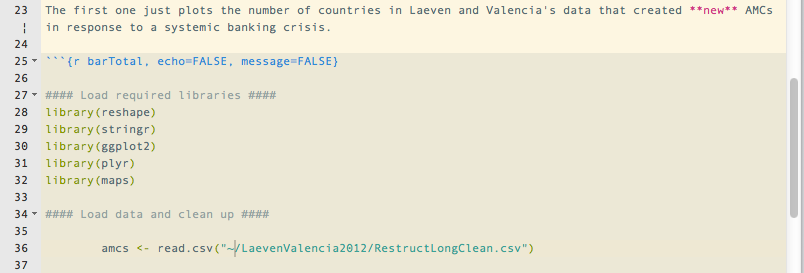
\includegraphics[width = \textwidth]{/git_repositories/Rep-Res-Book/Source/Children/Chapter3/images3/MarkdownNoCollapse.png}
    \end{subfigure} \\[0.5cm]
    
    \begin{subfigure}
        \caption{Folded}
      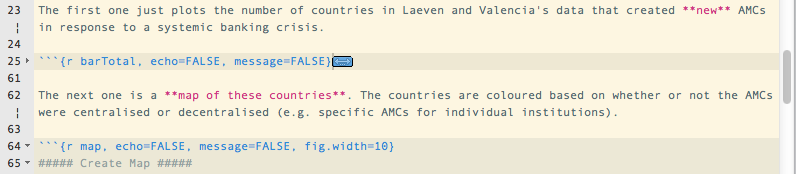
\includegraphics[width = \textwidth]{/git_repositories/Rep-Res-Book/Source/Children/Chapter3/images3/MarkdownCollapse.png}        
    \end{subfigure}
    \end{center}
\end{figure}

\paragraph{R LaTeX}

You can see in the final image in Figure \ref{SourcePanes} that many of the options for R LaTeX files are the same as R Markdown files. The key differences being that there is a \texttt{Compile PDF} icon instead of \texttt{Knit HTML}. Clicking this icon knits the file and creates a PDF file in your R LaTeX file's directory. There is also a \texttt{Format} icon next instead of \texttt{MD}. This actually inserts LaTeX formatting commands into your document for things such as section headings and bullet lists.


\paragraph{Change default .Rnw knitter}
By default RStudio is set up to use{\emph{Sweave}}\index{Sweave} for compiling LaTeX documents. To use {\emph{knitr}} instead of {\emph{Sweave}} when knitting \texttt{.Rnw} files in RStudio you should go to the {\bf{Options}} window\index{RStudio Options window}. Click on the \texttt{Sweave} button. Select \texttt{knitr} from the drop down menu for ``Weave files using:". Finally, click \texttt{Apply}. The {\bf{Options}} window is in different places depending on the version of RStudio you are using:

    \begin{itemize}
        \item {\bf{Mac}}: \texttt{RStudio} \textrightarrow\; \texttt{Preferences},
        \item {\bf{Windows \& Linux}}: \texttt{Tools} \textrightarrow\; \texttt{Options}.
    \end{itemize}

\subsection{knitr \& R}

As an R package, you can of course knit documents in regular R (or using the console in RStudio). All of the syntax in the document you are knitting is the same as before. But instead of clicking a {\tt{Compile PDF}} or {\tt{knit HTML}} button we use is {\tt{knit}} command. To knit our example Markdown file {\emph{Example.Rmd}} we first set the working directory (see Chapter \ref{DirectoriesChapter}) to the the folder where your {\emph{Example.Rmd}} file is located with the {\tt{setwd}} command. In this example I have it on my desktop.\footnote{Using the directory name {\tt{$\sim$/Desktop/}} is for Mac computers. Please use alternative syntax discussed in Chapter \ref{DirectoriesChapter} on other types of systems.}

\begin{knitrout}
\definecolor{shadecolor}{rgb}{0.969, 0.969, 0.969}\color{fgcolor}\begin{kframe}
\begin{alltt}
\hlfunctioncall{setwd}(\hlstring{"~/Desktop/"})
\end{alltt}
\end{kframe}
\end{knitrout}


\noindent Then I knit my file:

\begin{knitrout}
\definecolor{shadecolor}{rgb}{0.969, 0.969, 0.969}\color{fgcolor}\begin{kframe}
\begin{alltt}
\hlfunctioncall{knit}(input = \hlstring{"Example.Rmd"}, output = \hlstring{"Example.md"})
\end{alltt}
\end{kframe}
\end{knitrout}


\noindent Note that if you do not specify the output file {\emph{knitr}} will determine what the file should be. In this example it would come up with the same name and location.

If you try this example, you find that the {\emph{knit}} command only created a Markdown file and not an HTML file like clicking the RStudio {\tt{knit HTML}} did. Likewise, if you use {\tt{knit}} on a {\tt{.Rnw}} file you will only end up with a basic LaTeX {\tt{.tex}} file and not a compiled PDF. To convert the Markdown file into HTML you need to further run the {\tt{.md}} file through the {\tt{markdownToHTML}} command from the {\emph{markdown}} package, i.e.

\begin{knitrout}
\definecolor{shadecolor}{rgb}{0.969, 0.969, 0.969}\color{fgcolor}\begin{kframe}
\begin{alltt}
\hlfunctioncall{mardownToHTML}(file = \hlstring{"Example.md"}, output = \hlstring{"Example.html"})
\end{alltt}
\end{kframe}
\end{knitrout}


You can combine the knit and markdownToHTML steps using {\emph{knitr}}'s \texttt{knit2html} command like this:

\begin{knitrout}
\definecolor{shadecolor}{rgb}{0.969, 0.969, 0.969}\color{fgcolor}\begin{kframe}
\begin{alltt}
\hlfunctioncall{knit2html}(file = \hlstring{"Example.Rmd"}, output = \hlstring{"Example.html"})
\end{alltt}
\end{kframe}
\end{knitrout}


\noindent If we want to compile a {\tt{.tex}} file in R we run it through the {\tt{texi2pdf}} command in the {\emph{tools}} package. This package will run both LaTeX and \BibTeX to create a PDF with a bibliography (see Chapter \ref{LatexChapter} for more details on using \BibTeX for bibliographies). Here is a {\tt{texi2pdf}} example:

\begin{knitrout}
\definecolor{shadecolor}{rgb}{0.969, 0.969, 0.969}\color{fgcolor}\begin{kframe}
\begin{alltt}
\hlcomment{# Load tools package}
\hlfunctioncall{library}(tools)
\hlcomment{# Compile pdf}
\hlfunctioncall{texi2pdf}(file = \hlstring{"Example.tex"})
\end{alltt}
\end{kframe}
\end{knitrout}


Just like with \texttt{knit2html}, you can speed up this process by using the \texttt{knit2pdf} command to compile a PDF file from a \texttt{.Rnw} or \texttt{.Rtex} document.
 
\section{R/RStudio Tips}

Finally, here are a few other tips that make using R and RStudio a little easier.

\noindent In RStudio you can click on the {\bf{Help}} pane (by default at the lower right, see Figure \ref{BlankMain}) and enter the command you want help with into the search field.

\paragraph{Autocomplete}

In R and RStudio you do not have to type out every command, argument, object, or even directory name. After you start typing a command/argument/object/directory name you can hit the ``tab" key to automatically complete the word you started. The \index{autocomplete} function is particularly good in RStudio. Not only does it give you a list of words to choose from, but it also shows you an abbreviated version of the help file for commands and arguments.


